% estimate.tex
\documentclass[tikz,border=1pt]{standalone}
\usetikzlibrary {decorations.pathreplacing,calligraphy}
\begin{document}
	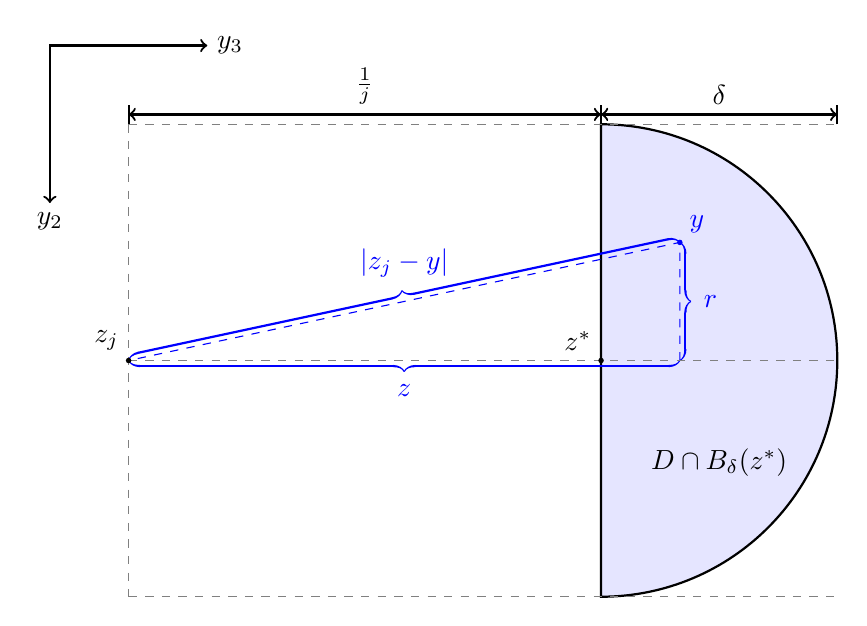
\begin{tikzpicture}
		% the half ball
		\filldraw[fill,fill opacity=0.5,color=blue!20,draw=black,thick] (0,-3) arc [start angle=-90, end angle=90, radius=3cm] -- cycle;
		
		% point y
		\fill[blue] (1,1.5) circle (1pt);
		\draw[blue] (1,1.5) node [above right] {$y$};
		\draw[dashed,blue] (1,0) -- (1,1.5) -- (-6,0);
		\draw[pen colour={blue},thick,decorate,decoration={calligraphic brace,amplitude=4pt}] (-6,0) -- (1,1.5) node[pos=0.5,above=5pt,blue]{$\vert z_{j} - y\vert$};
		\draw[pen colour={blue},thick,decorate,decoration={calligraphic brace,amplitude=4pt,mirror}] (-6,0) -- (1,0) node[pos=0.5,below=5pt,blue]{$z$};
		\draw[pen colour={blue},thick,decorate,decoration={calligraphic brace,amplitude=4pt,mirror}] (1,0) -- (1,1.5) node[pos=0.5,right=5pt,blue]{$r$};
		
		% dashed line
		\draw[dashed,color=gray] (-6,3) -- (3,3)
		                         (-6,-3) -- (3,-3) 
		                         (-6,0) -- (3,0) 
		                         (-6,3) -- (-6,-3);
		                         
		% point z_j
		\fill[black] (-6,0) circle (1pt);
		\draw (-6,0) node [above left] {$z_{j}$};
		
		% point z^*
		\fill[black] (0,0) circle (1pt);
		\draw (0,0) node [above left] {$z^{*}$};
		
		% length for geometry
		\draw[thick] (-6,3) -- (-6,3.25)
		             (0,3) -- (0,3.25)
		             (3,3) -- (3,3.25);
		\draw[thick,<->] (-6,3.125) -- (0,3.125); 
		\draw[thick,<->] (0,3.125) -- (3,3.125);
		\draw (-3, 3.125) node [above] {$\frac{1}{j}$};
		\draw (1.5,3.125) node [above] {$\delta$};
		\draw (1.5,-1) node [below] {$D \cap B_{\delta}(z^{*})$};
		
		% axis
		\draw[thick,<->] (-7,2) -- (-7,4) -- (-5,4);
		\draw (-5,4) node [right] {$y_{3}$};
		\draw (-7,2) node [below] {$y_{2}$};
	\end{tikzpicture}
\end{document}